
\documentclass[english]{pkuslide}

\usepackage[cmrgreekup]{def}

\addbibresource{TemplateBibliography.bib}

\newtheorem{Thm}{Thm}
\newtheorem{ColoredThm}{ColoredThm}

\definecolor{nonpkupurple}{HTML}{c71585}
\AtBeginEnvironment{ColoredThm}{%
\setbeamercolor{block title}{use=example text,fg=gray!10,bg=nonpkupurple!75!bg}%
}

\title[Dynamic Systems \& Deep Learning]{An Odyssey in Hamilton-Jacobi Equations}
\subtitle{Hopf-Lax Formula, Numerical Algorithms, and Link to Deep Learning}
\institute{Peking University}

\author{Yixuan Wang}
\date{\today}

\subject{Title}
\keywords{Hamilton-Jacobi equation, Hopf-Lax formula, ADMM, control theory, differential games, Pontryagin's Maximum Principle, dynamic systems, Method of Successive Approximations, gradient descent, back propagation, deep learning.}

	\begin{document}

	\begin{frame}
\titlepage
	\end{frame}

	\begin{frame}
\tableofcontents[subsectionstyle=show]
	\end{frame}

\section{Mathematical Background}
\frame{\sectionpage}
\subsection{Hamilton-Jacobi Equation}

	\begin{frame}{Definition}
\begin{alertblock}{Hamilton-Jacobi Equation}
\begin{equation}
\frac{\partial \varphi}{\partial t} + H(x,p,t) = 0  \qquad in\  \mathbb{R}^{d} \times (0,\infty) 
\end{equation}
\begin{equation}
\varphi(x,0) = g(x)  \qquad in\  \mathbb{R}^{d}
\end{equation}

\end{alertblock}
where \begin{math} x \in \mathbb{R}^{d}\end{math} denotes the state coordinate and \begin{math}t \in \mathbb{R} \end{math} denotes the time coordinate; \begin{math} H :  \mathbb{R}^{d} \times \mathbb{R}^{d} \times (0,\infty) \to \mathbb{R} \end{math} is a prescribed function called the Hamiltonian;  \begin{math} \varphi \coloneqq \varphi(x,t) : \mathbb{R}^{d} \times (0,\infty) \to \mathbb{R}  \end{math} is our target solution for the Hamilton-Jacobi Equation; \begin{math} p \coloneqq \nabla _{x}{\varphi} \end{math} denotes the gradient vector with respect to $x$; $g(x)$ is given as the initial data.
	\end{frame}

	\begin{frame}{Viscosity Solution}{Motivation}
We assume the Hamiltonian has the form of $H(p, x)$.

The original Hamilton-Jacobi equation can often be a fully nonlinear first-order PDE, so it is difficult to tackle. In the method of vanishing viscosity, we introduce a second-order term for regularization, converting it into a semilinear parabolic PDE as follows
\begin{equation}
\frac{\partial \varphi}{\partial t} + H(p, x) - \varepsilon \Delta_{x}{\varphi}  = 0  \qquad in\  \mathbb{R}^{d} \times (0,\infty) 
\end{equation}
where $\Delta_{x}{\varphi}$ denotes the Laplacian with respect to $x$, $\varepsilon$ is a constant and we denote the solution by $\varphi^\varepsilon$. As $\varepsilon \to 0$, we hope $\varphi^\varepsilon$ would converge to our weak solution $\varphi$, or at least in terms of a subsequence as Arzela-Ascoli theorem would imply.
	\end{frame}
\begin{frame}{Viscosity Solution}{Formulation}
\begin{exampleblock}{Viscosity Solution}
Assume $H$, $g$ are continuous. A bounded function $u$, which is uniformly continuous for each $T > 0$ in \begin{math} \mathbb{R}^{d} \times [0,T] \end{math}, is a viscosity solution provided that: (1) \begin{math} u(x,0) = g(x)  \  in\  \mathbb{R}^{d} \end{math}; (2) for all \begin{math} v \in C^\infty(\mathbb{R}^{d} \times (0,\infty)) \end{math}, if $u-v$ has a local maximum at $(x_0, t_0)$, then \begin{math} v_t{(x_0, t_0)} + H(\nabla _x{v(x_0, t_0), x_0)} \leq 0\end{math}; (3) \begin{math} v_t{(x_0, t_0)} + H(\nabla _x{v(x_0, t_0), x_0)} \geq 0\end{math} for a local minimum at $(x_0, t_0)$.
\end{exampleblock}
It can be verified that if $u$ is constructed using the method of vanishing viscosity, it indeed satisfies the previous condition.
	\end{frame}
	\begin{frame}{Viscosity Solution}{Consistency}
\begin{enumerate}[<+->]
\item A classical solution is clearly a viscosity solution.
\item If a viscosity solution $u$ is differentiable at $(x_0, t_0)$, then \begin{math} u_t{(x_0, t_0)} + H(\nabla _x{u(x_0, t_0), x_0)} = 0\end{math}.
\end{enumerate}
	\end{frame}
	\begin{frame}{Viscosity Solution}{Uniqueness}
\begin{Thm}[Uniqueness]
Suppose $H$ enjoys the Lipschitz continuity 
\begin{equation}
  \left\{
   \begin{array}{l}
   |H(p, x) - H(q, x)| \leq C|p-q|,  \\
   |H(p, x) - H(p, y)| \leq C|x-y|(1+|p|).  \\
   \end{array}
  \right.
\end{equation} 
Then there is at most one viscosity solution for the Hamilton-Jacobi equation
\begin{equation}
  \left\{
   \begin{array}{l}
  \frac{\partial \varphi}{\partial t} + H(p, x)  = 0  \qquad in\  \mathbb{R}^{d} \times (0, T] ,  \\
   \varphi(x,0) = g(x)  \qquad in\  \mathbb{R}^{d}.  \\
   \end{array}
  \right.
\end{equation} 
\end{Thm}
	\end{frame}
\subsection{Control Theory and Dynamic System}
\begin{frame}{Intro to Control Theory}
We have the following optimal control problem
\begin{equation}
  \left\{
   \begin{array}{l}
   \dot{x}(t) = f(x(t), \alpha(t)) \qquad t>0,  \\
   x(0) = x^0.  \\
   \end{array}
  \right.
\end{equation}
where $\alpha$ ($\alpha(t) \in A$) denotes a control from an admissible set \begin{math}\mathcal{A}\end{math}; $x$ denotes the response to the control according to our ODE. Now we wish to maximize the following payoff functional
\begin{equation}
P[\alpha(\cdot)] \coloneqq \int_{0}^{T} r(x(t), \alpha(t))dt +g(x(T))
\end{equation}
where $r$ and $g$ are given as the running payoff and the terminal payoff respectively; the terminal time $T > 0$ is given as well.
\end{frame}
\begin{frame}{Dynamic Programming} {Motivation}
When evaluating the integral
\begin{equation}
\int_{0}^{\infty} \frac{\sin x}{x} dx \nonumber
\end{equation}
We define 
\begin{equation}
I(\alpha) \coloneqq \int_{0}^{\infty} e^{-\alpha x} \frac{\sin x}{x} dx \nonumber
\end{equation}
Now since we can compute
\begin{equation}
I'(\alpha) = -\frac{1}{\alpha^{2}+1} \nonumber
\end{equation}
We can get that our integral equals $\frac{\pi}{2}$ since $I(\infty)$ equals $0$.
\end{frame}
\begin{frame}{Dynamic Programming} {Perspective}
Embed the optimal control problem into a larger family of similar problems, namely we vary the initial state and time of the controlled dynamics
\begin{equation}
  \left\{
   \begin{array}{l}
   \dot{x}(t) = f(x(t), \alpha(t)) \qquad s<t \leq T,  \\
   x(s) = x.  \\
   \end{array}
  \right.
\end{equation} 
with the target payoff functional
\begin{equation}
P_{x,s}[\alpha(\cdot)] \coloneqq \int_{s}^{T} r(x(t), \alpha(t))dt +g(x(T))
\end{equation}
Now we define the value function $v$ to be the greatest payoff starting at a given state and time
\begin{equation}
v(x,t)  \coloneqq \sup_{\alpha(\cdot) \in \mathcal{A}}{P_{x,t}[\alpha(\cdot)]}
\end{equation}
Note that $v(x,T)=g(x)$.
\end{frame}
\begin{frame}{Dynamic Programming} {Property of the Value function}
\begin{Thm}[Optimality Conditions]
For each $h>0$ $s.t$ $t+h\leq T$, we have
\begin{equation}
v(x, t)=\inf_{\alpha(\cdot) \in \mathcal{A}}{ \{ \int_{t}^{t+h}r(x(s), \alpha(s))ds +v(x(t+h), t+h)\}} 
\end{equation} 
where $x(\cdot)$ solves the ODE for the control $\alpha(\cdot)$.
\end{Thm}
\end{frame}
\begin{frame}{Dynamic Programming} {Derivation of the Equation}
\begin{Thm}[Hamilton-Jacobi-Bellman Equation]
Assume the value function $v$ is $C^1$. Then $v$ solves the PDE
\begin{equation}
v_{t}(x, t)+\max_{a \in A}{ \{ f(x, a)\cdot \nabla_{x}{v(x,t)} +r(x,a) \}} =0
\end{equation} 

\end{Thm}
Now we can define the Hamiltonian 
\begin{equation}
H(x,p) \coloneqq  \max_{a \in A}H(x,p,a) \coloneqq \max_{a \in A}{\{ f(x,a)\cdot p +r(x,a) \} }
\end{equation}
\end{frame}
\begin{frame}{Dynamic Programming} {Application}
Now we discuss how to solve the optimal control problem using the idea of dynamic programming.
\begin{enumerate}[<+->]
\item Firstly we solve the Hamilton-Jacobi-Bellman equation to compute value function $v$.
\item Then we use the value function to design $\alpha$ at each point, according to $\alpha(x,t)=a$, for the maximum in Hamiltonian to be attained.
\item Next we solve the control system of ODE, now that $\alpha$ can be expressed as a function of $x$ and $t$.
\item Finally we define the feed back control $\alpha(t) \coloneqq \alpha(x(t),t)$.
\end{enumerate}
\end{frame}
\begin{frame}{Pontryagin Maximum Principle}{Statement of the Theorem}
\begin{Thm}[Pontryagin Maximum Principle]
Assume $\alpha(\cdot)$ is optimal for our control problem, and $x(\cdot)$ is the corresponding trajectory. Then there exists a function \begin{math} p : [0,T] \to \mathbb{R}^{d} \end{math} such that
\begin{equation}
  \left\{
   \begin{array}{l}
  (ODE) \qquad \,\,\,\,\,\dot{x}(t) = \nabla_{p}{H}(x(t),p(t),\alpha(t)),  \\
   (I) \qquad \qquad \,\,\,\,x(0) = x^0,  \\
   (ADJ) \qquad\,\,\,\,\,\, \dot{p}(t) = -\nabla_{x}{H}(x(t),p(t),\alpha(t)),  \\
   (T) \qquad \qquad \,\,\,p(T) = \nabla g(x(T)),  \\
  (C) \qquad \qquad \,\,the\  mapping \quad t \mapsto H(x(t),p(t),\alpha(t)) \quad is \ constant, \\
   (M) \qquad \qquad H(x(t),p(t),\alpha(t))= \max_{a \in A}{H(x(t),p(t),a)} .  \\
   \end{array}
  \right.
\end{equation} 

\end{Thm}
\end{frame}
\begin{frame}{Pontryagin Maximum Principle}{Connection with Dynamic Programming}
If the value function defined in the dynamic programming process is $C^2$, then the costate $p(\cdot)$ in the Pontryagin Maximum Principle is given by
\begin{equation}
p(s) = \nabla_{x} v(x(s) ,s) \qquad  (t\leq s \leq T)
\end{equation}
\end{frame}
\begin{frame}{Pontryagin Maximum Principle} {Application}
Now we discuss how to solve the optimal control problem using the Pontryagin Maximum Principle.
\begin{enumerate}
\item We write out those PDE equations and solve $x(\cdot)$, $\alpha(\cdot)$, $p(\cdot)$ simultaneously.
\item We often utilize the maximum equation (M) to compute the control $\alpha(\cdot)$.
\end{enumerate}
\end{frame}
\begin{frame}{Miscellaneous Complements} 
\begin{enumerate}[<+->]
\item We can utilize dynamic programming method to derive Hamilton-Jacobi equations for solving differential games.
\item Without assuming value function $\in C^1$, we still have that $v$ is the unique viscosity solution to our Hamilton-Jacobi-Bellman Equation, provided that $g$,$r$,$f$ are bounded and Lipschitz continuous. In this way, we can formally obtain our value function by solving the PDE, since viscosity solution is unique.
\end{enumerate}
\end{frame}
\section{Hopf-Lax Type Formula}
	\frame{\sectionpage}
\subsection{Hopf-Lax Formula in its Simplest Form}
\begin{frame}{Characteristic Equations}{General Review}
\begin{ColoredThm}[Structure of Characteristic ODE]
\usebeamercolor{Thm title}
For a nonlinear first-order PDE $F(Du,u,x) = 0$, where $F$ is smooth, we have the following equations
\begin{equation}
  \left\{
   \begin{array}{l}
   (a)\ \dot{p}(s) = -D_{x}F(p(s),z(s),x(s))-D_{z}F(p(s),z(s),x(s))p(s), \\
    (b)\ \dot{z}(s) = D_{p}F(p(s),z(s),x(s))\cdot p(s), \\
    (c)\ \dot{x}(s) = D_{p}F(p(s),z(s),x(s)).  \\
   \end{array}
  \right.
\end{equation}
Assume a $C^2$ function $u$ solves the original PDE, and $\dot{x}(\cdot)$ solves the ODE (c), where $p(\cdot) \coloneqq Du(x(\cdot))$, $z(\cdot) \coloneqq u(x(\cdot))$, then $p(\cdot)$ solves (a) and $z(\cdot)$ solves (b).
\end{ColoredThm}

	\end{frame}
\begin{frame}{Characteristic Equations}{For Hamilton-Jacobi Equation}
For our Hamilton-Jacobi Equation $u_{t} + H(Du, x) = 0$, the characteristic equations become
\begin{equation}
  \left\{
   \begin{array}{l}
   \dot{x}= D_{p}H(p, x), \\
   \dot{p}= -D_{x}H(p, x), \\
\dot{z} = D_{p}H(p,x)\cdot p + H(p, x).  \\
   \end{array}
  \right.
\end{equation}
	\end{frame}
	\begin{frame}{Legendre Transform}{Definition}
\begin{exampleblock}{Convex Conjugate}
For a function \begin{math} f :  \mathbb{R}^{d} \to \mathbb{R} \cup \{ \infty \} \end{math}, we define its convex conjugate $f^{*}$ \begin{math}:\mathbb{R}^{d} \to \mathbb{R} \cup \{ \infty \} \end{math} as follows
\begin{equation}
 f^{*}(p) \coloneqq \sup \{\langle p, x\rangle -f(x) | x \in \mathbb{R}^{d} \}
\end{equation}
$f^{*}$ is also called the Legendre-Fenchel transformation of $f$.
\end{exampleblock}
If $L$ is convex, and $\lim_{|v| \to \infty}\frac{L(v)}{|v|}=+\infty$, then for $H=L^*$, $H$ is convex, and $\lim_{|p| \to \infty}\frac{H(p)}{|p|}=+\infty$. Moreover, $L=H^*$.
	\end{frame}
	\begin{frame}{Legendre Transform}{For Hamiltonian}
	Suppose now Hamiltonian $H=H(Du)$, the mapping $H$ is convex, and $\lim_{|p| \to \infty}\frac{H(p)}{|p|}=+\infty$. $L=H^*$.
	
	We notice that $L^{*}(p)= p\cdot v -L(v)$ implies the derivative of $r.h.s.$ $w.r.t.$ $v$ equals 0, since it reaches a maximum at $v$. Hence $DL(v)=p$. 
	
	Now we have that the following equations are equivalent
	\begin{equation}
  \left\{
   \begin{array}{l}
   v= DH(p), \\
   p= DL(v), \\
   p\cdot v = L(v)+ H(p).  \\
   \end{array}
  \right.
\end{equation}
	\end{frame}
	\begin{frame}{Hopf-Lax Formula}{Formulation}
	Now let's return to our problem of Hamilton-Jacobi equation. The method of characteristics implies $\dot x$ = $DH(p)$, and $\dot z$ = $DH(p) \cdot p -H(p)$. As a result, $\dot z=L(\dot x)$, which provides a clue for our following definition.
	\begin{exampleblock}{Hopf-Lax Formula}
Assume additionally that the initial data $g(\cdot)$ is Lipschitz continuous, we define $u(x,t)$ as follows
\begin{equation}
u(x,t) \coloneqq \inf \{\int_{0}^{t}L(\dot w(s))ds +g(w(0)) | w(t)=x \}
\end{equation}
\end{exampleblock}
	\end{frame}
	\begin{frame}{Hopf-Lax Formula}{Properties}
	\begin{enumerate}[<+->]
\item $u$ is Lipschitz continuous, thus differentiable $a.e.$.
\item \begin{math} u(x,0)=g(x)  \end{math}.
\item \begin{math} u(x,t) = \min_{y \in \mathbb{R}^{d}} \{ tL(\frac{x-y}{t})+g(y) \} \end{math}.
\item  \begin{math} u(x,t) = \min_{y \in \mathbb{R}^{d}} \{ (t-s)L(\frac{x-y}{t-s})+u(y,s) \} \qquad for \ 0 \leq s <t \end{math}.
\item $u$ satisfies the Hamilton-Jacobi equation at points where it is differentiable.
\end{enumerate}
	\end{frame}
	\begin{frame}{Hopf-Lax Formula}{Uniqueness}
	The uniqueness of a weak solution can be guaranteed if we impose a semi-concavity restriction, which is indeed satisfied by our Hopf-Lax formula provided that $g$ is semiconcave or $H$ is uniformly convex.
	\end{frame}
	\begin{frame}{Hopf-Lax Formula}{Uniqueness}
	\begin{Thm}[Semi-concavity]
	If there exists a constant $C$, s.t \begin{math} g(x+z)-2g(x)+g(x-z) \leq c |z|^2\end{math},
	
	then \begin{math} u(x+z,t)-2u(x,t)+u(x-z,t) \leq c |z|^2\end{math},
        
	Or, if there exists a constant $\theta >0$, s.t. \begin{math} \sum_{i,j=1}^{n}H_{p_{i}p_{j}}(p)\xi_{i}\xi_{j} \geq \theta |\xi|^2 \qquad for\  all\  p, \xi \in \mathbb{R}^{d} \end{math},
	
	then \begin{math} u(x+z,t)-2u(x,t)+u(x-z,t) \leq \frac{1}{\theta t} |z|^2\end{math}.
	\end{Thm}
		\end{frame}
	\begin{frame}{Hopf-Lax Formula}{Uniqueness}
	\begin{Thm}[Semi-concavity]
	If $u$ solves the initial value problem $a.e.$, and \begin{math} u(x+z,t)-2u(x,t)+u(x-z,t) \leq C(1+\frac{1}{t}) |z|^2\end{math} for some constant $C$, then $u$ is unique.
	\end{Thm}
	\end{frame}
	\begin{frame}{Additional Comment}
\begin{enumerate}[<+->]
\item Hopf-Lax formula gives us a viscosity solution.
\item We can view Hopf-Lax formula as a special case of dynamic programming.
\end{enumerate}
	\end{frame}

\subsection{Generalized Hopf-Lax Formula}
\begin{frame}{Time-dependent Case}{Formulation}
Consider the Hamilton-Jacobi equation
\begin{equation}
\frac{\partial \varphi}{\partial t} + H(p,t) = 0  \qquad in\  \mathbb{R}^{d} \times (0,T) 
\end{equation}
\begin{equation}
\varphi(x,T) = g(x)  \qquad in\  \mathbb{R}^{d}
\end{equation}
where $g$ is convex.

Note that we are considering Hamilton-Jacobi equation given the terminal state for the sake of consistency with reference materials, reversing it back in time would give us a Hamilton-Jacobi equation we originally considered.
\end{frame}
\begin{frame}{Time-dependent Case}{Assumption}
Define \begin{math} S=\{ s \in \mathbb{R}^{d} : |s|=1\}    \end{math}, 

\qquad\ \ \,\begin{math}B_{+}=\{(s,r) \in \mathbb{R}^{d} \times \mathbb{R} : |s|^2+r^2\leq 1, r>0\}\end{math}.

We have the following assumptions on Hamiltonian
\begin{enumerate}[<+->]
\item $H$ is continuous in $t \in (0,T)$ for every \begin{math}s \in \mathbb{R}^{d}\end{math}.
\item $H$ is summable on $(0,T)$ for every \begin{math}s \in \mathbb{R}^{d}\end{math}.
\item For all $(t,s) \in (0,T)\times S$, $\lim_{r \to 0^{+}}rH(\frac{s}{r},t)=H_{0}(s,t)$ exists and $H_{0}(s,\cdot)$ is continuous on $(0,T)$ for every $s \in S$.
\item For all $t \in (0,T)$, $(s_1,r_1), (s_2,r_2) \in B_{+}$, and for some constant $L$, $|r_{1}H(\frac{s_{1}}{r_{1}},t)-r_{2}H(\frac{s_{2}}{r_{2}},t)| \leq L(|s_{1}-s_{2}|^2+(r_{1}-r_{2})^2)^{\frac{1}{2}}$.
\end{enumerate}
\end{frame}
\begin{frame}{Time-dependent Case}{Hopf-Lax Formula}
We give the following theorem when the Hamiltonian is dependent on time $t$, without formally state the exact definition of minimax solutions.
\begin{Thm}[Hopf-Lax Formula in Time-dependent Case]
For mild assumptions on terminal data $g$ and Hamiltonian $H$, we have
 \begin{equation}
v(x,t) = \sup_{s \in \mathbb{R}^{d}}\{\langle s,x \rangle+\int_{t}^{T}H(s,r)dr-g^{*}(s)\}
\end{equation}
the formula above gives a minimax solution. 
	\end{Thm}
	\ 
	
Namely, $v(x,t)=\bigg( g^{*}(s)-\int_{t}^{T}H(s,r)dr\bigg) ^{*}(x)$.
\end{frame}
\begin{frame}{Time-dependent Case}{Further assumptions}
The "mild assumptions" in the statement of the theorem could be 
\begin{enumerate}[<+->]
\item $H(\cdot,t)$ is convex (or concave) in $s$ for every $t$.
\item The maximizer in our formula for $v$ is unique for all $(s,t)$. As is a special case when $g$ is an affine function.
\end{enumerate}
\end{frame}
\begin{frame}{Function-dependent Case}{Formulation}
Consider the Hamilton-Jacobi equation
\begin{equation}
\frac{\partial V}{\partial t} + H(t,V,p) = 0  \qquad in\  \mathbb{R}^{d} \times (0,T) 
\end{equation}
\begin{equation}
V(T, x) = \varphi(x)  \qquad in\  \mathbb{R}^{d}
\end{equation}
We would not go into the details of the Hopf-Lax formula for this type of equation, see the reference material for more information.
\end{frame}

\begin{frame}{Additional Comment}
\begin{enumerate}[<+->]
\item minimax solutions and viscosity solutions are in fact equivalent.
\item The above Hopf-Lax Formulas are natural generalizations of the prototype.
\end{enumerate}
\end{frame}

\section{Algorithms for Numerical Computation}
	\frame{\sectionpage}
\subsection{Hopf-Lax Type Conjecture}
\begin{frame}{Comments in Advance}
\begin{enumerate}[<+->]
\item Let's look at the optimality condition. In this situation, the conjecture is a natural generalization of Hopf-Lax formula using the idea of dynamic programming.
\item The formulas coincide with the time-dependent Hopf-Lax formula when the Hamiltonian is independent of the current state.
\end{enumerate}

\end{frame}
	\begin{frame}{Lax Type Conjecture}
\begin{figure}
\centering
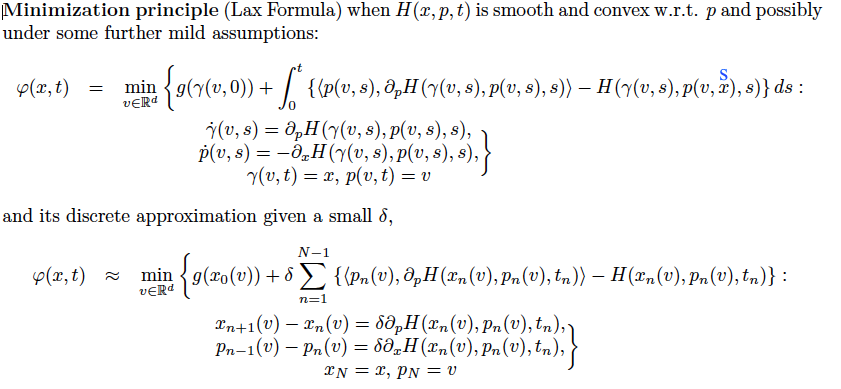
\includegraphics[height=0.5\textheight]{1.png}
\end{figure}
	\end{frame}
\begin{frame}{Lax Type Conjecture}
\begin{figure}
\centering
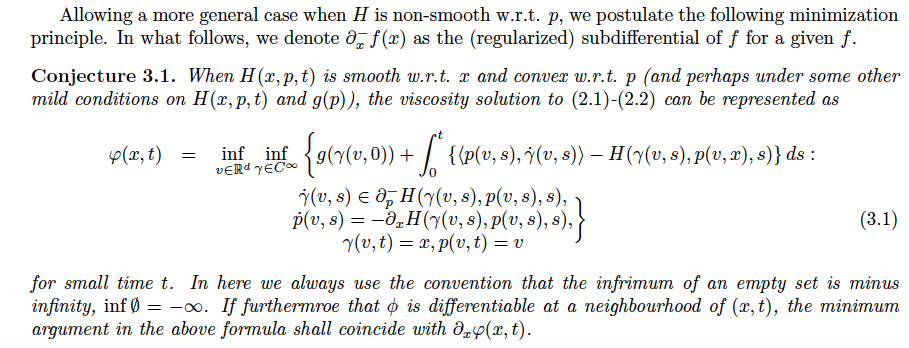
\includegraphics[height=0.5\textheight]{2.png}
\end{figure}

	\end{frame}
	\begin{frame}{Hopf  Type Conjecture}
\begin{figure}
\centering
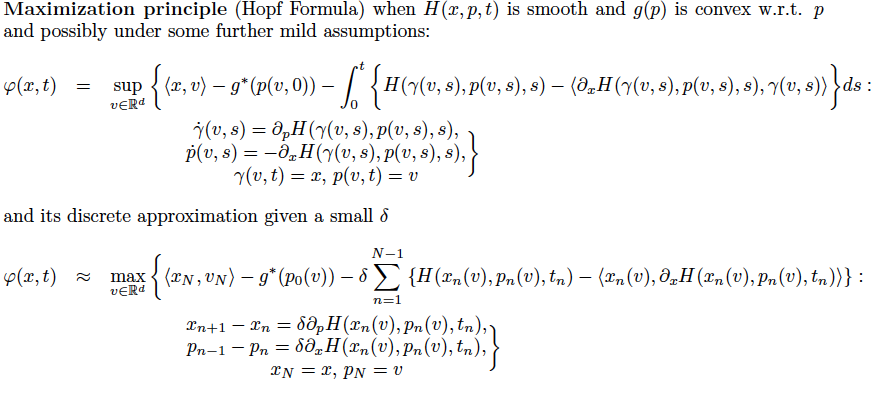
\includegraphics[height=0.5\textheight]{3.png}
\end{figure}
	\end{frame}
\begin{frame}{Hopf Type Conjecture}
\begin{figure}
\centering
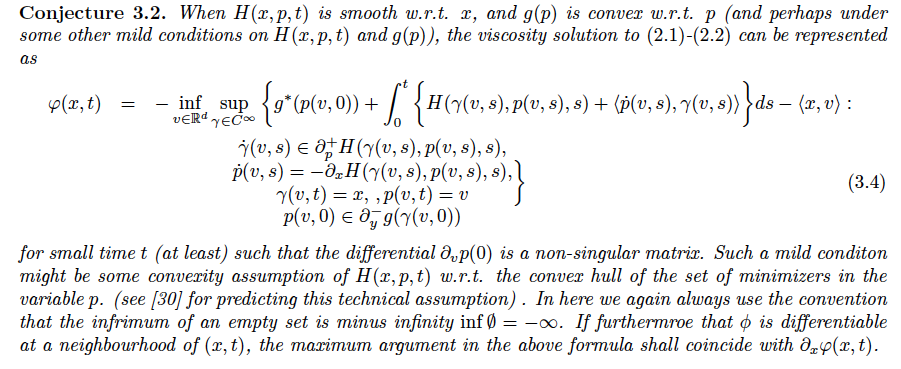
\includegraphics[height=0.5\textheight]{4.png}
\end{figure}

	\end{frame}
\subsection{Design of Algorithms}
	\begin{frame}{Objective function}
	We wish to minimize the following functions (Lax and Hopf type conjecture respectively)
	\begin{figure}
\centering

\includegraphics[height=0.1\textheight]{5.png}

\centering
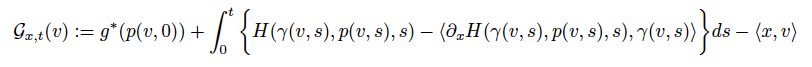
\includegraphics[height=0.1\textheight]{6.png}
\end{figure}
subject to the following restriction
\begin{figure}
\centering
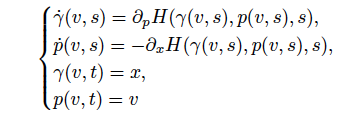
\includegraphics[height=0.2\textheight]{7.png}
\end{figure}
\end{frame}
\begin{frame}{Optimization method}
We perform the following method of gradient descent
\begin{figure}
\centering
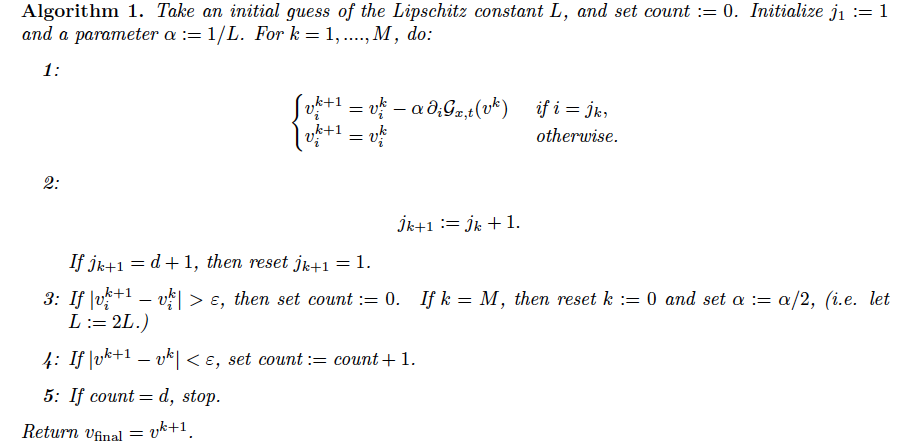
\includegraphics[height=0.5\textheight]{8.png}
\end{figure}
where the gradient could be taken by numerical differentiation, and the ODE could be solved numerically.
\end{frame}
\begin{frame}{Optimization method for ordinary Hopf-Lax Formula}
For our Hopf-Lax formula 
 \begin{equation}
\varphi(x,t) = -\min_{v \in \mathbb{R}^{d}}\{tH(v)+J^{*}(v)-\langle v,x \rangle\}
\end{equation}
We can use the following ADMM algorithm for optimization
\begin{figure}
\centering

\includegraphics[height=0.5\textheight]{9.png}
\end{figure}

\end{frame}
\section{Connection with Deep Learning}

	\frame{\sectionpage}

	\begin{frame}{Intuition}
\nocite{*} 
Since the ultimate goal of machine learning is to create a class of functions that can represent the data with desired accuracy, our aim is to approximate a target function with minimum loss. 

In this perspective, we view deep learning and convolutional neural networks as discrete dynamic systems.
We can use continuous
	\end{frame}

%\section{Quote slides}

% To test slide quotes, one may make a copy of the output and rename
% it to be pkuslideTemplateQuote.pdf
\IfFileExists{pkuslideTemplateQuote.pdf}{
	\begin{quoteslide}
\includepdf[pagecommand=\quotefootnote{Some footnote}, pages=1, scale=0.8]{pkuslideTemplateQuote.pdf}
	\end{quoteslide}
}
{}

\section{Acknowledgements}
\subsection{Bibliography}
	\begin{frame}{Reference : Books and Techreports}
\printbibliography[type = book]
\printbibliography[keyword = aaa]
	\end{frame}
\begin{frame}{Reference : Articles}
\printbibliography[type = article]
	\end{frame}

\subsection{Complimentary Close}

	\begin{frame}
\LARGE
\begin{beamercolorbox}[center, ht=3em]{titlelike}
\vspace{1em}
Thanks!
\end{beamercolorbox}
	\end{frame}

	\end{document}
